% !TEX encoding = UTF-8 Unicode

\documentclass[a4paper]{article}

\usepackage{color}
\usepackage{url}
\usepackage[T2A]{fontenc} % enable Cyrillic fonts
\usepackage[utf8]{inputenc} % make weird characters work
\usepackage{graphicx}
\usepackage[document]{ragged2e}
\usepackage{}
\usepackage[english,serbian]{babel}
\usepackage[
    style=numeric,
    sorting=none
]{biblatex}
\addbibresource{seminarski.bib}

\usepackage[unicode]{hyperref}
\hypersetup{colorlinks,citecolor=green,filecolor=green,linkcolor=blue,urlcolor=blue}



\begin{document}
\title{Svemir kao velika neuronska mreža\\ \small{Seminarski rad u okviru kursa\\Tehničko i naučno pisanje\\ Matematički fakultet}}

\author{Aleksa Filipović, Marta Kiso, Veljko Seničanin, Luka Stamenković\\stamenkovicl777@gmail.com}
\date{15.~novembar 2022.}
\maketitle
\abstract{\justifying{
U ovom radu ćemo diskutovati o mogućnosti da je ceo univerzum jedna velika neuronska mreža. Samu ideju je dao ruski naučnik Vitali Vančurin sa Univerziteta u Minesoti u svom naučnom radu. \cite{1}
\\Princip kog ćemo pokušati da se držimo jeste taj da ne zalazimo previše u oblasti fizike i astronomije, već da na što jednostavniji način pokušamo da približimo ovu temu čitaocima. Opisaćemo šta je to neuronska mreža, kao i da li i na koji način je možemo povezati sa kosmososom.
}}
\tableofcontents

\newpage

\section{Uvod}
\label{sec:uvod}
\justifying
Kako bismo uopšte mogli da razmatramo opciju da se svemir može zamisliti kao neuronska mreža, važno je da tačno definišemo šta je to neuronska mreža. U uvodu ćemo je posmatrati iz biološkog ugla, dok ćemo u narednom poglavlju diskutovati o neuronskoj mreži u vidu implementacije sistema veštačke inteligencije. Neuronska mreža predstavlja nervni sistem živih bića, u bukvalnom smislu je to jedan veliki skup povezanih nervnih ćelija - neurona.  

Astronomi su pokušali da utvrde razlike i sličnosti dva najsloženija nama poznata sistema, mada u potpuno različitim razmerama – svemira i njegovih galaksija i mozga i njegovih neuronskih ćelija. Ispostavilo se da su sličnosti mnogo veće nego što se moglo pretpostaviti. Okupljeni u timu, astorfizičari, neurolozi i neurohirurzi su otkrili da su, i pored toga što su razmere neuporedive, strukture mozga i svemira izuzetno slične. U nekim aspektima, ova dva sistema izgledaju sličnija jedan drugom, nego delovima koji ih čine.  

Navodi se da izuzetno različiti fizički procesi dovode do vrlo sličnih složenih i organizovanih struktura. Na primer, ljudski mozak deluje zahvaljujući mreži od skoro 70 milijardi neurona koji ga zajedno čine. Analogno, pretpostavlja se da svemir ima najmanje 100 milijardi galaksija.\cite{6} Oba ova sistema su organizovana u složenu mrežu povezanu dugim nitima i čvorovima koji ih povezuju Ovi čvorovi se uočavaju na slikama i svemira i mozga, što objašnjava neke očigledne sličnosti. Konkretno, na slici \ref{fig:komparacija} možemo vrlo lako uvideti sličnost.

\begin{figure}[h!]
\begin{center}
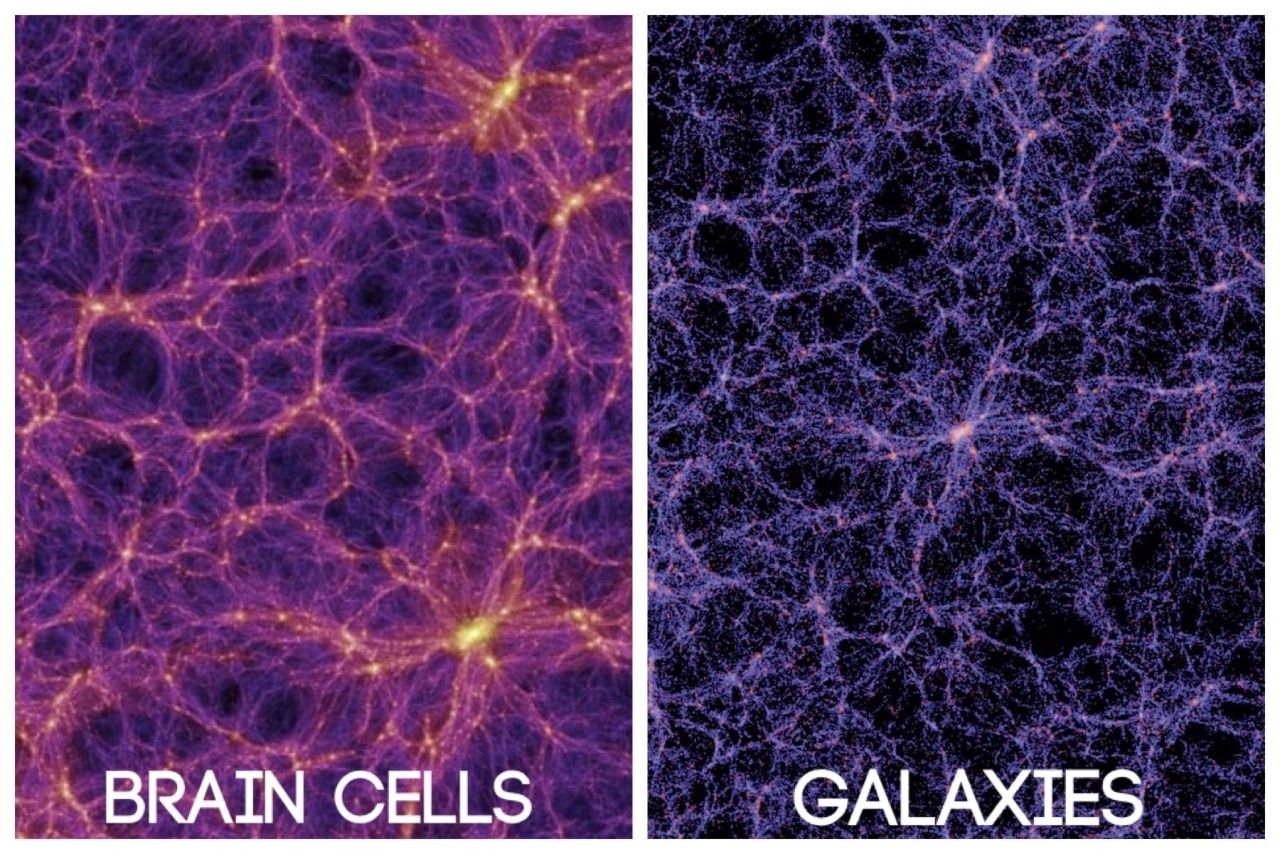
\includegraphics[scale=0.2]{komparacija.jpeg}
\end{center}
\caption{Komparacija ćelija mozga i galaksija}
\label{fig:komparacija}
\end{figure}

\justifying
Takođe, u oba sistema, ove mreže čine samo 30 odsto mase. U svakom od njih oko 70 odsto mase zapravo čine delovi za koje se čini da su pasivni: moždana tečnost i tamna materija svemira.

Vitali Vančurin misli da ako posmatramo svemir kao neuronsku mrežu, njegovo ponašanje pod određenim uslovima možemo objasniti jednačinama kvantne mehanike i zakonima klasične fizike, poput teorije relativnosti koju je osmislio Albert Ajnštajn. Vačurin smatra da bi daljim proučavanjem ove teorije mogao rešiti glavni problem moderne fizike \--\ neslaganje klasične mehanike,
koja opisuje kako svemir funkcioniše u velikim razmerima i kvantne mehanike koja se bavi proučavanjem atomskog i subatomskog nivoa materije.  Kao što je poznato, razlika između klasične i kvantne mehanike jeste ta što je u klasičnoj mehanici vreme apsolutno i univerzalno, dok je u kvantnoj mehanici relativno.

 Vančurin je u intervjuu za časopis \textit{Futurism} \cite{7} istakao ključnu tačku svog rada. Naime, on je zaključio da je dinamika učenja neuronskih mreža veoma slična kvantnoj dinamici u fizici. Ono što je zapravo rečeno je da je učenje neuronskih mreža u nekim granicama logična, dok izvan tih granica ne važe ista pravila kao unutar njih. To se može uporediti sa zakonima klasične i kvantne mehanike. Najbolje bi to bilo predstaviti u tabeli \ref{tab:tabela1}
 
\begin{table}[h!]
\begin{center}
\rowcolors{2}{gray!10}{gray!40}
\begin{tabular}{|c|c|} \hline
Klasična fizika& Kvantna fizika\\ \hline
Telo poseduje ili čestična ili talasna svojstva & Telo poseduje i čestična i talasna svojstva\\ 
Možemo tačno odrediti i poziciju i brzinu tela &Nemoguće je tačno odrediti\\ 
Ne postoji dilatacija vremena& Postoji dilatacija vremena \\ 
Ne postoji kontrakcija dužine& Postoji kontrakcija dužine\\ \hline
\end{tabular}
\caption{Razlike između klasične i kvantne fizike}
\label{tab:tabela1}
\end{center}
\end{table}


\printbibliography[
heading=bibintoc,
title={Literatura}
]

\end{document}


